% Apresentação de andamento do TCC ao orientador.
% Compilar: cd docs/apresentacao && pdflatex tcc-andamento.tex && pdflatex tcc-andamento.tex
% Gráficos leem os dados do benchmark em ../relatorios/dados/ (gerados por bench/orquestracao/agregar.py).
% Imagens vêm de ../pesquisa/img/.
\documentclass[11pt,aspectratio=169]{beamer}
\usepackage[utf8]{inputenc}
\usepackage[T1]{fontenc}
\usepackage[brazil]{babel}
\usepackage{lmodern}
\usepackage{booktabs}
\usepackage{tabularx}
\usepackage{graphicx}
\usepackage{pgfplots}
\usepackage{pgfplotstable}
\usepackage{listings}
\usetikzlibrary{arrows.meta,positioning,calc,shapes.misc}
\pgfplotsset{compat=1.18}
\graphicspath{{../pesquisa/img/}}

% ---------- Cores (acento do NarraTer, escurecido para fundo claro) ----------
\definecolor{acento}{HTML}{6D5BD0}
\definecolor{tinta}{HTML}{1F2330}
\definecolor{suave}{HTML}{5B6170}
\definecolor{linha}{HTML}{D9DCE3}
\definecolor{fundo}{HTML}{F5F5F8}
\definecolor{ok}{HTML}{2E8B57}
\definecolor{ruim}{HTML}{C0392B}
\definecolor{alerta}{HTML}{B7791F}
\definecolor{cDevA}{HTML}{3D7DD8}
\definecolor{cDevB}{HTML}{2E9E6B}

% ---------- Tema mínimo ----------
\usefonttheme{professionalfonts}
\setbeamertemplate{navigation symbols}{}
\setbeamercolor{normal text}{fg=tinta}
\setbeamercolor{frametitle}{fg=tinta}
\setbeamercolor{title}{fg=tinta}
\setbeamercolor{structure}{fg=acento}
\setbeamercolor{alerted text}{fg=acento}
\setbeamerfont{frametitle}{size=\Large,series=\bfseries}
\setbeamerfont{title}{size=\LARGE,series=\bfseries}
\setbeamertemplate{itemize items}{\raisebox{0.15ex}{\small$\bullet$}}
\setbeamertemplate{enumerate items}[default]
\setbeamertemplate{frametitle}{%
  \vspace*{0.5em}\insertframetitle\par
  \vspace*{-0.2em}{\color{acento}\rule{2.2em}{2pt}}\vspace*{0.1em}}
\setbeamertemplate{footline}{%
  \leavevmode\hbox to\paperwidth{\hspace*{1.2em}{\color{suave}\tiny NarraTer · andamento do TCC}\hfill
  {\color{suave}\tiny\insertframenumber/\inserttotalframenumber}\hspace*{1.2em}}\vspace*{0.6em}}
\setbeamertemplate{section page}{%
  \vfill{\color{acento}\rule{3em}{3pt}}\par\vspace{0.6em}
  {\usebeamerfont{title}\insertsectionhead\par}\vfill}
\AtBeginSection{\begin{frame}[plain,noframenumbering]\sectionpage\end{frame}}

% Rótulos de evidência (D09)
\newcommand{\ev}[2]{{\scriptsize\sffamily\colorbox{#1!12}{\textcolor{#1!80!black}{[#2]}}}}
\newcommand{\medido}{\ev{ok}{medido}}
\newcommand{\observado}{\ev{cDevA}{observado}}
\newcommand{\citado}{\ev{suave}{citado}}
\newcommand{\inferido}{\ev{alerta}{inferido}}
\newcommand{\cmd}[1]{\texttt{\color{acento!80!black}#1}}

\lstset{basicstyle=\ttfamily\scriptsize, columns=fullflexible, keepspaces=true,
  backgroundcolor=\color{fundo}, frame=none, xleftmargin=4pt, xrightmargin=4pt,
  aboveskip=4pt, belowskip=4pt, showstringspaces=false, breaklines=true,
  literate={á}{{\'a}}1 {é}{{\'e}}1 {í}{{\'i}}1 {ó}{{\'o}}1 {ú}{{\'u}}1 {ã}{{\~a}}1
           {õ}{{\~o}}1 {ç}{{\c c}}1 {ê}{{\^e}}1 {â}{{\^a}}1 {Ã}{{\~A}}1 {→}{{$\to$}}1 {·}{{$\cdot$}}1}

\pgfplotsset{
  bench/.style={
    width=\linewidth, height=5.4cm,
    xtick={0,...,7}, xticklabels={A,B,C,D,E,E-sl0,F,G},
    xmin=-0.6, xmax=7.6, ymin=0,
    ymajorgrids, grid style={linha},
    axis line style={suave}, tick style={suave},
    tick label style={font=\scriptsize}, label style={font=\scriptsize},
    legend style={font=\scriptsize, draw=none, fill=none},
  },
  milhoes/.style={y filter/.code={\pgfmathparse{##1/1000}}},
}

\title{Quando a orquestração de agentes de IA compensa?\\[2pt]{\Large Um estudo empírico com o NarraTer}}
\subtitle{Andamento do Trabalho de Conclusão de Curso}
\author{Gabriel Cortez}
\date{12 de novembro de 2026}

\begin{document}

\begin{frame}[plain]
\vfill
{\color{acento}\rule{3em}{3pt}}\par\vspace{0.8em}
{\usebeamerfont{title}\inserttitle\par}
\vspace{0.6em}{\large\color{suave}\insertsubtitle\par}
\vspace{1.6em}
{\insertauthor\par}
{\small\color{suave}\insertdate\par}
\vfill
\end{frame}

\begin{frame}{Roteiro}
\begin{enumerate}
\setlength\itemsep{0.45em}
\item De onde o trabalho partiu, e como a pergunta mudou
\item O que a literatura diz sobre orquestrar agentes
\item O instrumento: o NarraTer e como ele produz evidência
\item Fase exploratória: tornar a orquestração confiável e medível
\item O experimento central: equipe contra agente sozinho, em duas tarefas
\item Da evidência à ferramenta: o portão, o gerador de equipes e o aceite
\item Limitações, próximos passos e perguntas ao orientador
\end{enumerate}
\end{frame}

\section{De onde partimos}

\begin{frame}{Agentes de código vivem em terminais isolados}
\begin{columns}[T]
\begin{column}{0.55\linewidth}
\begin{itemize}
\setlength\itemsep{0.6em}
\item Os agentes de programação mais usados hoje são \textbf{programas de terminal}: Claude Code, Codex,
  Gemini CLI, OpenCode.
\item Cada um é de um fornecedor, com sua interface e seus formatos internos.
\item Eles não conversam entre si. Quem passa contexto de um para outro é a pessoa, copiando e colando.
\item Quando um fornecedor oferece times de agentes, só funciona \textbf{dentro do próprio produto}.
\end{itemize}
\end{column}
\begin{column}{0.42\linewidth}
\centering
\begin{tikzpicture}[
  term/.style={draw=linha, fill=fundo, rounded corners=3pt, minimum width=2.6cm, minimum height=0.9cm, font=\scriptsize},
  >=Stealth]
\node[term] (a) at (0,2.4) {Claude Code};
\node[term] (b) at (0,1.2) {Codex};
\node[term] (c) at (0,0) {Gemini CLI};
\node[font=\Large] (p) at (-2.6,1.2) {\textcolor{suave}{?}};
\draw[<->, suave, dashed] (a) -- (b) node[midway,right,font=\tiny] {?};
\draw[<->, suave, dashed] (b) -- (c) node[midway,right,font=\tiny] {?};
\node[font=\scriptsize, text width=2.8cm, align=center, color=suave] at (0,-1.1) {cada um no seu terminal, sem protocolo comum};
\end{tikzpicture}
\end{column}
\end{columns}
\end{frame}

\begin{frame}{Como a pergunta mudou}
\centering
\begin{tikzpicture}[>=Stealth,
  fase/.style={draw=linha, fill=fundo, rounded corners=3pt, align=left, font=\scriptsize, anchor=north, inner sep=5pt},
  data/.style={font=\scriptsize\bfseries, color=acento}]
\draw[->, suave, thick] (-0.3,0) -- (14.4,0);
\foreach \x/\d in {1.6/{julho}, 5.4/{outubro}, 9.2/{15/10}, 12.8/{16/10}}
  { \fill[acento] (\x,0) circle (2.2pt); \node[data, above] at (\x,0.08) {\d}; }
\node[fase] at (1.6,-0.3) {\parbox[t][2.9cm][t]{3.2cm}{\raggedright\textbf{\small Uma ferramenta}\\[3pt]
  Fazer agentes de fornecedores diferentes (Claude, Gemini, Codex) conversarem num canvas.\\[3pt]
  \textcolor{ruim}{Modelo cooperativo: só funcionou com o Claude.}}};
\node[fase] at (5.4,-0.3) {\parbox[t][2.9cm][t]{3.2cm}{\raggedright\textbf{\small Um protocolo}\\[3pt]
  O terminal como API universal (D01). Para funcionar, foi preciso \textbf{medir}: quando o agente terminou?
  A resposta chega inteira?}};
\node[fase] at (9.2,-0.3) {\parbox[t][2.9cm][t]{3.2cm}{\raggedright\textbf{\small Um benchmark}\\[3pt]
  Sete versões, 24 rodadas. Todas tiraram nota máxima; o que mudava era o \textbf{custo de coordenar}.}};
\node[fase, draw=acento, line width=1pt] at (12.8,-0.3) {\parbox[t][2.9cm][t]{3.2cm}{\raggedright\textbf{\small Uma pergunta}\\[3pt]
  Se a nota não muda e só o custo muda: \textbf{um agente sozinho não faria igual?}
  Quando a orquestração compensa?}};
\end{tikzpicture}
\vspace{0.6em}

\begin{block}{}
\small Construir a ferramenta antes de fechar a teoria foi uma \textbf{fase exploratória}: foi ela que revelou a
pergunta certa e produziu o instrumento para respondê-la.
\end{block}
\end{frame}

\begin{frame}{Pergunta de pesquisa}
\begin{block}{}
\large \textbf{Quando} a orquestração de vários agentes de IA compensa, em relação a \textbf{um agente
sozinho}, em tarefas de programação? E como uma ferramenta pode \textbf{decidir} isso?
\end{block}
\vspace{0.6em}
\begin{description}[Q3]
\setlength\itemsep{0.35em}
\item[Q1] Em que tipo de tarefa uma equipe ganha de um agente sozinho, em \textbf{nota, tempo e custo}?
\item[Q2] \textbf{De onde vem} o custo de coordenar: do protocolo, da forma da equipe ou do tamanho das partes?
\item[Q3] Que \textbf{regra} uma ferramenta deve seguir para montar, ou não montar, uma equipe?
\end{description}
\vspace{0.4em}
{\small\color{suave} Pré-requisito, já resolvido na fase exploratória: uma orquestração entre agentes de qualquer
fornecedor que saiba quando o agente terminou e receba a resposta inteira.}
\end{frame}

\begin{frame}{O que a literatura diz}
\scriptsize
\begin{tabularx}{\linewidth}{@{}l X@{}}
\toprule
Fonte & Achado \\
\midrule
\textbf{MAST} (Cemri et al., 2025) & 14 modos de falha em sistemas multiagente: projeto do sistema $\sim$44\%,
  desalinhamento entre agentes $\sim$32\%, \textbf{verificação} $\sim$23,5\%. \\
\textbf{Kim et al.} (Google/MIT, 2025) & 180 configurações: coordenar ganha 80,8\% em tarefas
  \textbf{paralelizáveis} e perde 39--70\% nas \textbf{sequenciais}; acima de $\sim$45\% de acerto do agente
  sozinho, coordenar não compensa. \\
\textbf{Vals.ai} (2026) & Equipes construindo apps: custo de 1,8$\times$ a 5,1$\times$; ganho significativo em
  1 de 4 configurações. \\
\textbf{Tran e Kiela} (2026) & Com o mesmo orçamento de tokens, o agente sozinho empata ou ganha. \\
\textbf{Anthropic} (2025) & Multiagente vale em pesquisa ampla e paralela, a $\sim$15$\times$ os tokens; código
  é um encaixe ruim. \\
\textbf{Cognition} (2025--26) & ``Não construa multiagentes'': a escrita deve ficar numa linha só. O que funciona
  é um \textbf{revisor com contexto limpo}. \\
\bottomrule
\end{tabularx}
\vspace{0.5em}

{\footnotesize\citado{} Números principais conferidos na fonte (\texttt{docs/pesquisa/orquestracao.md}).\\
\inferido{} Hipótese: em tarefas que um agente forte resolve sozinho, a equipe só acrescenta custo.}
\end{frame}

\begin{frame}{Ferramentas relacionadas}
\footnotesize
\begin{tabularx}{\linewidth}{@{}l X X l@{}}
\toprule
Projeto & Como sabe que o agente terminou & Como obtém a resposta & Exige cooperação? \\
\midrule
Maestri (macOS) & tela & tela & não \\
Orca & \emph{hooks} em $\sim$25 CLIs + regras de tela em JSON + título da janela & ferramenta \texttt{worker-read}, blocos de 1.200 caracteres & sim \\
CLI Agent Orchestrator (AWS) & expressões regulares por CLI sobre a tela & tela & não \\
Agent Teams (Claude Code) & evento interno do programa & mensagem empurrada & só Claude \\
\midrule
\textbf{NarraTer} & tela + título + \emph{transcript} quando existe & \emph{transcript}, ou tela & \textbf{não} \\
\bottomrule
\end{tabularx}
\vspace{0.6em}

{\scriptsize\color{suave} Estudos em \texttt{docs/pesquisa/} (código-fonte lido em versões e \emph{commits} registrados).
A literatura acadêmica está no slide anterior.}
\end{frame}

\section{O instrumento: NarraTer}

\begin{frame}{O NarraTer: um canvas de terminais}
\begin{columns}[c]
\begin{column}{0.60\linewidth}
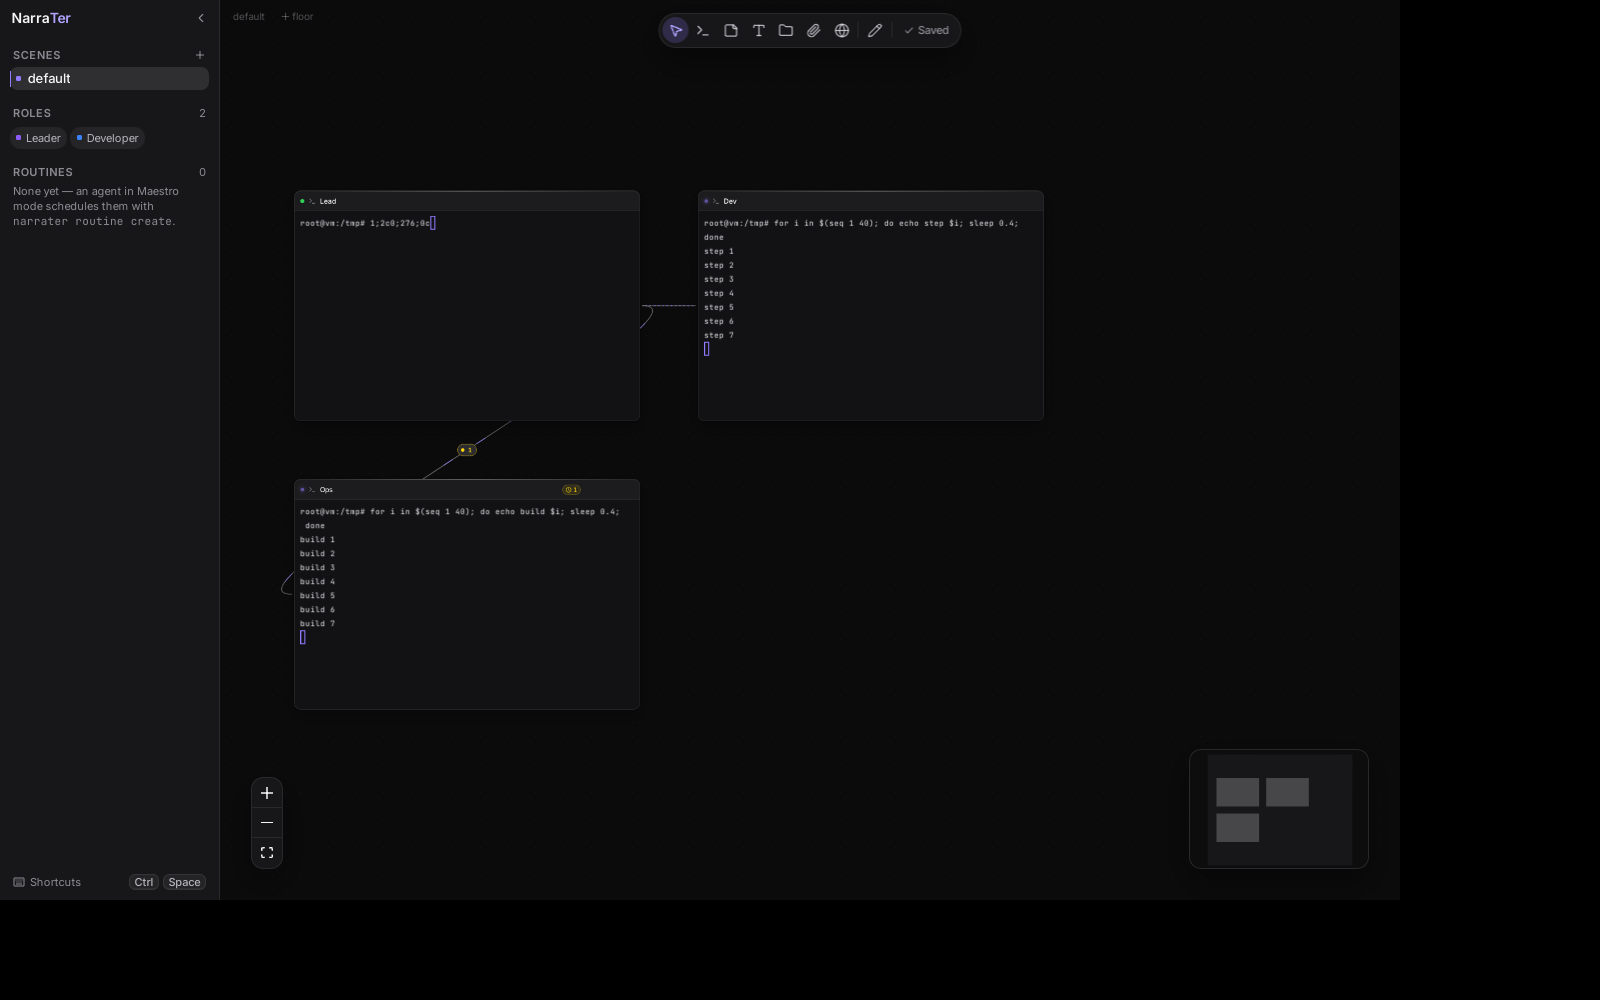
\includegraphics[width=\linewidth, trim=220 0 200 0, clip]{narrater-depois-ativo.png}
\end{column}
\begin{column}{0.38\linewidth}
\small
\begin{itemize}
\setlength\itemsep{0.5em}
\item Aplicativo para Linux (Tauri 2: Rust + React).
\item Cada \textbf{nó} é um terminal real (um PTY).
\item Cada \textbf{aresta} é uma permissão: quem pode falar com quem.
\item Os agentes conversam por uma CLI, \cmd{narrater}, que o app instala.
\item O estado de cada terminal (trabalhando, pronto, precisa de você) vem da tela.
\end{itemize}
\end{column}
\end{columns}
\end{frame}

\begin{frame}[fragile]{Exemplo: um líder delega a um desenvolvedor}
\begin{columns}[T]
\begin{column}{0.47\linewidth}
O Narrador (líder) roda no seu terminal:
\begin{lstlisting}[breaklines=false]
$ narrater ask DevA "Implemente a
    conversão de moedas e rode os testes.
    Responda com o resultado."
\end{lstlisting}
\vspace{0.3em}
E recebe de volta a resposta final do DevA:
\begin{lstlisting}[breaklines=false]
Implementei a funcionalidade multimoeda
e os testes passam (43 testes, OK). As
alterações estão em pedidos/cambio.py,
modelo.py ...
\end{lstlisting}
\vspace{0.3em}
{\scriptsize\color{suave} O DevA não instalou nada nem conhece protocolo: o pedido foi digitado no terminal dele.}
\end{column}
\begin{column}{0.50\linewidth}
\centering
\begin{tikzpicture}[>=Stealth, font=\scriptsize,
  lane/.style={draw=linha, fill=fundo, rounded corners=2pt, minimum width=1.7cm, minimum height=0.6cm, font=\scriptsize\bfseries},
  msg/.style={->, thick}, y=0.62cm]
\node[lane] (n) at (0,0) {Narrador};
\node[lane] (b) at (2.4,0) {NarraTer};
\node[lane] (d) at (4.8,0) {DevA};
\foreach \x in {0,2.4,4.8} \draw[linha, thick] (\x,-0.6) -- (\x,-8.6);
\draw[msg, acento] (0,-1.2) -- node[above] {\cmd{ask DevA}} (2.4,-1.2);
\node[right, align=left, color=suave, font=\tiny] at (2.45,-1.8) {aresta existe? (\texttt{resolve\_target})};
\node[right, align=left, color=suave, font=\tiny] at (2.45,-2.3) {espera o DevA ficar ocioso};
\draw[msg, acento] (2.4,-3.4) -- node[above] {digita o pedido} (4.8,-3.4);
\draw[cDevA, line width=3pt] (4.8,-3.6) -- (4.8,-6.0);
\node[right, color=cDevA, font=\tiny] at (4.9,-4.8) {trabalha};
\node[right, align=left, color=suave, font=\tiny] at (2.45,-4.4) {lê a tela (200 ms)};
\node[right, align=left, color=suave, font=\tiny] at (2.45,-4.9) {e o \emph{transcript}};
\draw[msg, suave, dashed] (4.8,-6.4) -- node[above] {fim do turno} (2.4,-6.4);
\draw[msg, acento] (2.4,-7.4) -- node[above] {resposta final} (0,-7.4);
\end{tikzpicture}
\end{column}
\end{columns}
\end{frame}

\begin{frame}{A tese central: o terminal é a API universal (decisão D01)}
\begin{columns}[T]
\begin{column}{0.48\linewidth}
\textbf{Julho: modelo cooperativo}
\begin{itemize}\small
\item Servidor MCP, \emph{prompt} de sistema extra, \emph{hook} de parada.
\item O alvo responde por ID com uma ferramenta própria.
\item \textcolor{ruim}{Só funcionava com o Claude Code.} Um alvo que não conhece o protocolo trava o pedido até o \emph{timeout}.
\end{itemize}
\end{column}
\begin{column}{0.48\linewidth}
\textbf{Outubro: modelo agnóstico}
\begin{itemize}\small
\item O estado do turno é lido da \textbf{tela renderizada} (emulador vt100 sem interface).
\item O pedido é digitado quando o alvo está ocioso.
\item Instruções chegam por arquivo (\texttt{CLAUDE.md}, \texttt{AGENTS.md}), que toda CLI lê.
\item \textcolor{ok}{Qualquer programa que roda num terminal participa.}
\end{itemize}
\end{column}
\end{columns}
\vspace{0.8em}
\begin{block}{Regra derivada (D05/D06)}
Cooperação do agente só entra como \textbf{opcional que melhora o resultado}. Se o agente não cooperar, tudo
continua funcionando pela tela.
\end{block}
\end{frame}

\begin{frame}[fragile]{Registro de decisões com evidência classificada (D09)}
\begin{columns}[T]
\begin{column}{0.44\linewidth}
\small
Cada decisão com alternativa real vira uma entrada em \texttt{docs/decisoes.md} (24 até agora), com seis campos:
\begin{itemize}\setlength\itemsep{0.2em}
\item contexto, decisão;
\item alternativas recusadas e por quê;
\item evidência \textbf{rotulada}:\\
  \medido{} \observado{} \citado{} \inferido{}
\item consequência;
\item \textbf{condição que derrubaria a decisão}.
\end{itemize}
\vspace{0.3em}
{\scriptsize\color{suave} O arquivo só cresce: uma decisão revista ganha entrada nova que cita a antiga.}
\end{column}
\begin{column}{0.54\linewidth}
\begin{lstlisting}[basicstyle=\ttfamily\tiny]
## D20 · A resposta do ask e o fim do turno vêm
##       do transcript do agente quando ele existe

Alternativas consideradas.
- Scrollback do emulador: o Claude Code roda em
  tela alternativa, o histórico é vazio [medido]
- Usar só o end_turn: o bloco de pensamento traz
  end_turn 15 s antes do texto [observado]

Evidência.
- [medido] acha a resposta certa em 126 de 126
  pedidos das rodadas C a G
- [medido] asks prontos antes da hora:
  D 4 de 27, E 12 de 31, F e G 0 de 40

Revisar se: o Claude Code mudar o formato do
transcript; o benchmark voltar a mostrar asks
antes da hora ou respostas trocadas.
\end{lstlisting}
\end{column}
\end{columns}
\end{frame}

\begin{frame}{Regra de método: medir contra o programa real (D12)}
\begin{itemize}
\setlength\itemsep{0.6em}
\item Toda regra que lê a tela de um agente é testada contra o \textbf{programa real}, nunca contra uma tela lembrada.
\item Cada execução medida é gravada (asciicast) e vira \textbf{teste de regressão}: \texttt{tests/transcripts/} tem
  gravações reais do Claude Code (resposta curta, longa, ferramenta silenciosa, diálogo de permissão\dots).
\item A verdade vem de um \textbf{oráculo independente da tela}, ligado só no avaliador:
  \begin{itemize}\small
  \item shell: o próprio comando grava um \emph{timestamp} ao terminar;
  \item Claude Code: \emph{hooks} \texttt{Stop} e \texttt{PermissionRequest}, configurados só na medição.
  \end{itemize}
\item O app continua sem \emph{hooks}: o oráculo mede, não participa (D01 preservada).
\end{itemize}
\end{frame}

\begin{frame}{Verificabilidade: o painel Activity (D21)}
\begin{columns}[c]
\begin{column}{0.42\linewidth}
\centering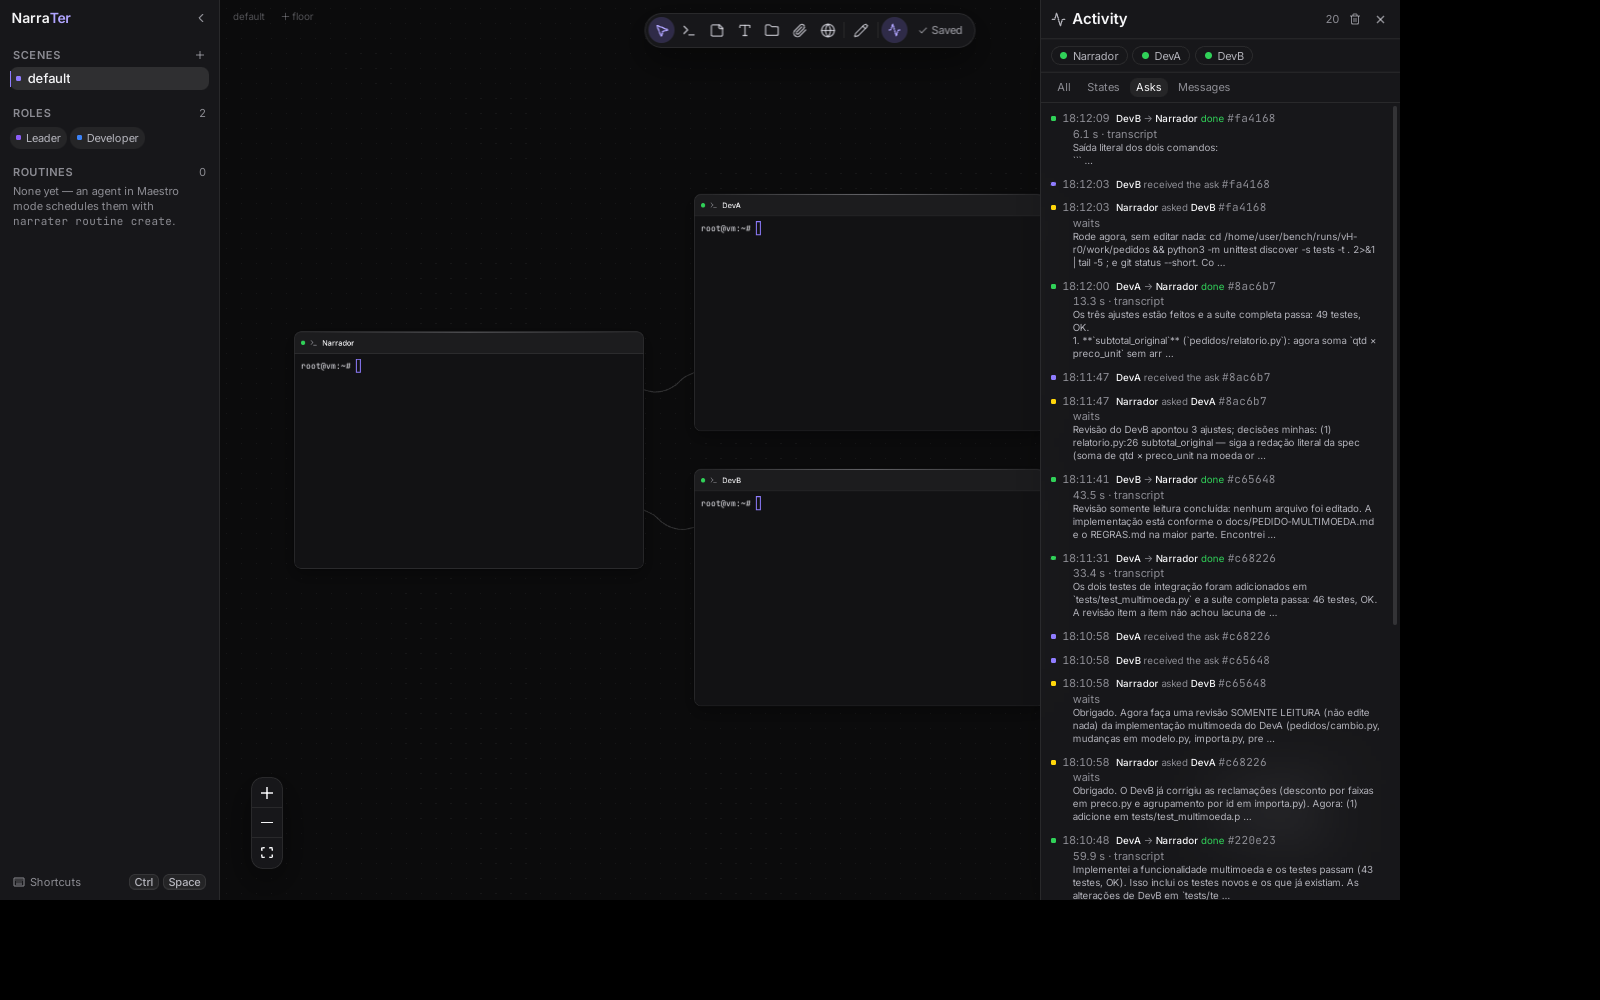
\includegraphics[height=0.8\textheight, trim=1040 280 200 0, clip]{painel-atividade.png}
\end{column}
\begin{column}{0.54\linewidth}
\small
\begin{itemize}\setlength\itemsep{0.5em}
\item Cada estado, pedido, entrega e resposta é gravado \textbf{pelo backend}, no momento em que acontece
  (\texttt{activity.jsonl}).
\item Nenhum agente escreve nesse registro: é o fato, não a palavra da IA.
\item Cada resposta mostra a duração e a \textbf{origem} (transcript ou tela).
\item Serve para auditar uma orquestração depois, e para explicar falhas como o ask antes da hora.
\end{itemize}
\end{column}
\end{columns}
\end{frame}

\section{Fase exploratória: tornar a orquestração confiável e medível}

\begin{frame}{Método: latência contra o oráculo}
\centering
\begin{tikzpicture}[>=Stealth, font=\small]
\draw[->, suave, thick] (0,0) -- (12,0) node[right] {tempo};
\draw[acento, thick] (1,-0.2) -- (1,0.2) node[above, align=center, font=\scriptsize] {pedido\\entregue};
\fill[cDevA!25] (1,-0.12) rectangle (7,0.12);
\node[font=\scriptsize, color=cDevA] at (4,-0.45) {agente trabalhando};
\draw[ok, very thick] (7,-0.35) -- (7,0.35) node[above, align=center, font=\scriptsize] {fim real\\(oráculo)};
\draw[acento, very thick, dashed] (8.2,-0.35) -- (8.2,0.35) node[above, align=center, font=\scriptsize] {detector\\diz ``pronto''};
\draw[<->, acento] (7,-0.8) -- node[below, font=\scriptsize] {latência $> 0$: correto} (8.2,-0.8);
\draw[ruim, very thick, dashed] (4.2,-0.35) -- (4.2,0.35) node[above, align=center, font=\scriptsize] {detector\\cedo demais};
\draw[<->, ruim] (4.2,-1.4) -- node[below, font=\scriptsize] {latência $< 0$: \textbf{prematuro} (resposta pela metade)} (7,-1.4);
\end{tikzpicture}
\vspace{0.6em}
\begin{itemize}\small
\item Detector = o próprio código do app (\texttt{screen.rs}), no mesmo ciclo de 200 ms.
\item Cenários: shell silencioso, com saída contínua, rajada + silêncio (direto e dentro do tmux); Claude Code com
  resposta curta, ferramenta silenciosa, resposta longa e pedido de permissão.
\item Ferramenta: \cmd{cargo run --release --example turn\_eval -- --reps N [--claude]}
\end{itemize}
\end{frame}

\begin{frame}{Resultados: antes e depois das correções (D10, D11)}
\footnotesize
\resizebox{\linewidth}{!}{\begin{tabular}{@{}l c c c c@{}}
\toprule
& \multicolumn{2}{c}{Antes} & \multicolumn{2}{c}{Depois} \\
\cmidrule(lr){2-3}\cmidrule(l){4-5}
Cenário & corretos/prem. (n) & latência & corretos/prem. (n) & latência \\
\midrule
shell direto (3 cenários) & 9 / 0 (9) & 0,6--0,8 s & 30 / 0 (30) & 0,6--0,8 s \\
tmux, saída contínua & 3 / 0 (3) & 0,76 s & 10 / 0 (10) & 0,75--0,78 s \\
\textbf{tmux, comando silencioso} & \textcolor{ruim}{0 / 3 (3)} & \textcolor{ruim}{$-$3,2 s} & \textcolor{ok}{10 / 0 (10)} & 0,6--0,8 s \\
\textbf{tmux, rajada + silêncio} & \textcolor{ruim}{0 / 3 (3)} & \textcolor{ruim}{$-$2,2 s} & \textcolor{ok}{10 / 0 (10)} & 0,8 s \\
Claude, turnos normais & 9 / 0 (9) & mediana 1,36 s & 15 / 0 (15) & mediana 0,55 s \\
\textbf{Claude, permissão} & \textcolor{ruim}{nunca detectado} & --- & \textcolor{ok}{3 / 0 (3)} & 0,1--0,2 s \\
\bottomrule
\end{tabular}}
\vspace{0.8em}

\medido{} Claude, turnos normais: antes n=9, depois n=15, faixas sem sobreposição
(Mann--Whitney exato, $p \approx 1{,}5\times10^{-6}$). tmux silencioso: 6/6 prematuros antes, 0/20 depois
(Fisher exato, $p \approx 4{,}3\times10^{-6}$).

{\scriptsize\color{suave} Ressalvas: uma máquina, uma versão do Claude Code (2.1.299, modelo Haiku); Codex e Gemini não medidos.}
\end{frame}

\begin{frame}{Desenho experimental (D19)}
\begin{columns}[T]
\begin{column}{0.52\linewidth}
\footnotesize
\textbf{Tarefa}: um repositório Python inventado (\texttt{pedidos}, $\sim$300 linhas) com regras de negócio próprias.
\begin{itemize}\setlength\itemsep{0.2em}
\item implementar pedidos em várias moedas (atravessa 3 módulos);
\item corrigir 2 defeitos descritos só como reclamação de cliente;
\item manter e escrever testes.
\end{itemize}
\textbf{Julgamento}: 31 \textbf{testes escondidos} que os agentes nunca veem, em 4 níveis. Solução de referência: 31/31.
Repositório inicial: 5/31.
\vspace{0.3em}

{\scriptsize\color{suave} Uma calculadora foi recusada: o modelo sabe o exercício de cor.}
\end{column}
\begin{column}{0.45\linewidth}
\footnotesize
\textbf{Equipe fixa}:
\begin{itemize}\setlength\itemsep{0.1em}
\item Narrador (líder, não edita): Claude Opus 5.5
\item DevA: Claude Sonnet 5.5
\item DevB: Claude Haiku 5.5
\end{itemize}
\textbf{Controles}:
\begin{itemize}\setlength\itemsep{0.1em}
\item toda rodada começa \textbf{zerada} (HOME, sessões, tmux, pasta);
\item mesma versão do Claude Code em todas;
\item \textbf{ordem contrabalançada} (o \emph{cache} do servidor dura 1~h);
\item 3 rodadas por versão;
\item métricas tiradas das transcrições, não do que o agente diz.
\end{itemize}
\end{column}
\end{columns}
\end{frame}

\begin{frame}{As versões comparadas: cada uma é um \emph{commit} real}
\small
\begin{tabularx}{\linewidth}{@{}l l X@{}}
\toprule
& Commit & O que muda \\
\midrule
\textbf{A} & \texttt{e708d7b} & Cooperativo (julho): MCP, \emph{prompt} de sistema, \emph{hook}. Só Claude. O dev envia o relatório inteiro. \\
\textbf{B} & \texttt{16cee0e} & Agnóstico (D01): CLI + \emph{skill}; o \texttt{ask} devolve a tela do alvo. \\
\textbf{C} & \texttt{95fb11a} & \texttt{ask} assíncrono e durável. \\
\textbf{D} & \texttt{db3d535} & Leitor de estado novo (Estudo 1) e \emph{statusline}. \\
\midrule
\textbf{E} & \texttt{8e2e5fa} & A resposta vem do \emph{transcript} do agente, não da tela. \quad \textbf{E-sl0}: E sem \emph{statusline} (ablação). \\
\textbf{F} & \texttt{26e3c06} & O \emph{transcript} também decide se o turno acabou. \\
\textbf{G} & \texttt{c6ba63e} & Cada \texttt{ask} acha o próprio turno (corrige pedidos paralelos). \\
\bottomrule
\end{tabularx}
\vspace{0.6em}

{\small A--D mediram a história do projeto. E--G foram criadas \textbf{a partir do diagnóstico} de A--D, cada uma corrigindo
uma falha vista nas rodadas da anterior.}
\end{frame}

\begin{frame}{O resultado que mudou a pergunta: a qualidade bateu no teto}
\begin{columns}[c]
\begin{column}{0.5\linewidth}
\centering
{\fontsize{44}{48}\selectfont\color{acento}\textbf{24/24}}\par
\vspace{0.3em}
{\small rodadas de equipe passaram em \textbf{31 de 31} testes escondidos}
\end{column}
\begin{column}{0.48\linewidth}
\small
\begin{itemize}\setlength\itemsep{0.5em}
\item \medido{} Todas as versões, todas as rodadas, nota máxima. O líder nunca editou um arquivo.
\item O que separava as versões era só o \textbf{custo}: tokens, tempo, quantas vezes o líder voltava aos devs.
\item A comparação era sempre \textbf{equipe contra equipe}. Faltava o grupo de controle:
  \textbf{um agente sozinho} na mesma tarefa.
\end{itemize}
\end{column}
\end{columns}
\end{frame}

\begin{frame}{O custo de coordenar mudou entre versões}
\begin{columns}[T]
\begin{column}{0.5\linewidth}
\centering
\begin{tikzpicture}
\begin{axis}[bench, ylabel={tokens processados (milhões)}, milhoes]
\addplot[only marks, mark=*, mark size=1.8pt, suave, fill opacity=0.6, draw opacity=0.6]
  table[x=idx, y=processados_k, col sep=comma] {../relatorios/dados/rodadas.csv};
\addplot[only marks, mark=-, mark size=7pt, ultra thick, acento]
  table[x=idx, y=processados_k, col sep=comma] {../relatorios/dados/versoes.csv};
\end{axis}
\end{tikzpicture}
\end{column}
\begin{column}{0.5\linewidth}
\centering
\begin{tikzpicture}
\begin{axis}[bench, ylabel={custo de API equivalente (US\$)}]
\addplot[only marks, mark=*, mark size=1.8pt, suave, fill opacity=0.6, draw opacity=0.6]
  table[x=idx, y=custo_usd, col sep=comma] {../relatorios/dados/rodadas.csv};
\addplot[only marks, mark=-, mark size=7pt, ultra thick, acento]
  table[x=idx, y=custo_usd, col sep=comma] {../relatorios/dados/versoes.csv};
\end{axis}
\end{tikzpicture}
\end{column}
\end{columns}
\vspace{-0.3em}
{\small Cada ponto é uma rodada; o traço é a média. \medido{} De A até D o custo \textbf{subiu} (1,8 $\to$ 3,4 milhões de
tokens; US\$\,0,69 $\to$ 1,02). Com F e G ele voltou ao nível da A (US\$\,0,65 e 0,74), \textbf{sem} prender o
NarraTer a um fornecedor.}
\end{frame}

\begin{frame}{Por que D custou mais? O mecanismo encontrado}
\begin{columns}[T]
\begin{column}{0.52\linewidth}
\centering
\begin{tikzpicture}
\begin{axis}[bench, height=5.2cm, ybar=0pt, bar width=5pt, ylabel={ocorrências (soma de 3 rodadas)},
  legend columns=1, legend style={at={(0.5,1.03)}, anchor=south}]
\addplot[fill=ruim!75, draw=none] coordinates {(0,0) (1,2) (2,6) (3,7) (4,3) (5,0) (6,1) (7,0)};
\addplot[fill=alerta!80, draw=none] coordinates {(0,0) (1,0) (2,1) (3,4) (4,12) (5,3) (6,0) (7,0)};
\legend{pedidos repetidos (resposta cortada), asks prontos antes da hora}
\end{axis}
\end{tikzpicture}
{\tiny\color{suave} ``Antes da hora'' só é medível a partir da C.}
\end{column}
\begin{column}{0.46\linewidth}
\footnotesize
\medido{} A latência do protocolo é de segundos (entrega 0,2--0,5~s; detecção 1,6--3,1~s). A duração cresce em
\textbf{minutos}: o que cresce é o número de pedidos do líder (3--5 na A, 7--10 na D).
\vspace{0.5em}

Duas falhas fazem o líder pedir de novo:
\begin{enumerate}\setlength\itemsep{0.2em}
\item \textbf{resposta cortada}: a tela mostra $\sim$13 linhas, e o relatório do dev é maior;
\item \textbf{ask antes da hora}: o leitor dava o turno por encerrado 4--5~s após a entrega, antes de o agente começar.
\end{enumerate}
\medido{} Na rodada E2, 8 de 16 asks voltaram cedo; o líder deixou de confiar no \texttt{ask}: 14 pedidos e 10 minutos.
\end{column}
\end{columns}
\end{frame}

\begin{frame}[fragile]{Exemplo real: o \texttt{end\_turn} que mente}
\small
Trecho do \emph{transcript} da rodada E2 (hoje é um teste em \texttt{tests/transcripts/}), resumido:
\begin{lstlisting}
15:40:32.7  user       "[narrater from Narrador]: Projeto: .../pedidos. NÃO altere nada..."
15:40:35.3  assistant  tool_use  Bash
15:40:37.3  user       tool_result
15:40:47.7  assistant  thinking            stop_reason = end_turn     <- parece o fim
15:41:03.1  assistant  text "Não alterei nada. Li REGRAS.md, ..."  stop_reason = end_turn
15:41:03.2  system     turn_duration                                    <- fim de verdade
\end{lstlisting}
\vspace{0.4em}
\begin{itemize}\setlength\itemsep{0.3em}
\item \observado{} O Claude Code grava cada bloco da mensagem como um registro, e todos levam o \texttt{stop\_reason}.
  O pensamento já diz \texttt{end\_turn} \textbf{15~s antes} de a resposta existir.
\item O fim confiável é o registro \texttt{system/turn\_duration}. A versão F passou a esperar por ele.
\item É formato interno do fornecedor e pode mudar: por isso a tela continua como reserva e o benchmark é o alarme.
\end{itemize}
\end{frame}

\begin{frame}{As falhas do protocolo foram a zero}
\small
\begin{tabular}{@{}l c c c c c@{}}
\toprule
& A (cooperativo) & D & E & F & G \\
\midrule
Asks prontos antes da hora & --- & 4/27 & 12/31 & \textcolor{ok}{\textbf{0/16}} & \textcolor{ok}{\textbf{0/24}} \\
Pedidos repetidos (por rodada) & 0, 0, 0 & 1, 5, 1 & 0, 2, 1 & 0, 1, 0 & \textcolor{ok}{\textbf{0, 0, 0}} \\
Pedidos do líder aos devs & 3--5 & 7--10 & 5--14 & 3--7 & 3--6 \\
Tokens processados (milhões) & 1,84 & 3,44 & 2,94 & 1,73 & 2,50 \\
Custo médio (US\$) & 0,69 & 1,02 & 0,97 & 0,65 & 0,74 \\
Prende a um fornecedor? & \textcolor{ruim}{sim} & não & não & não & não \\
\bottomrule
\end{tabular}
\vspace{0.8em}

\begin{itemize}\setlength\itemsep{0.3em}
\item \medido{} D contra G: sem sobreposição em tokens, custo e pedidos (Mann--Whitney exato, U~=~9, $p = 0{,}10$, o
  menor $p$ possível com 3 contra 3).
\item \medido{} O leitor de \emph{transcript} acha a resposta certa em 126 de 126 pedidos reais das rodadas C--G.
\item \inferido{} O que ainda separa G de A é o ritmo dos agentes, não a coordenação: na G3, 243~s foram o DevB (Haiku)
  trabalhando sem parar.
\end{itemize}
\end{frame}

\section{O experimento central: equipe contra agente sozinho}

\begin{frame}{Desenho: o braço ``sozinho''}
\setbeamerfont{itemize/enumerate body}{size=\footnotesize}
\begin{columns}[T]
\begin{column}{0.56\linewidth}
\footnotesize
\textbf{Mesmo benchmark}, mesma tarefa, mesmos testes escondidos, mesmas condições (rodada zerada, 3 por montagem).
Muda só \textbf{quem trabalha}:
\begin{itemize}\setlength\itemsep{0.3em}
\item \textbf{Sozinho}: um terminal, Claude Opus 5.5, o mesmo pedido.
\item \textbf{Equipe}: Narrador (Opus) + DevA (Sonnet) + DevB (Haiku), versões F e G do protocolo, já sem
  as falhas da fase exploratória.
\end{itemize}
\vspace{0.3em}
Duas tarefas:
\begin{itemize}\setlength\itemsep{0.3em}
\item \texttt{pedidos}: funcionalidade que atravessa 3 módulos + 2 defeitos (31 testes);
\item \texttt{armazem}: \textbf{4 módulos independentes}, feita para a equipe ganhar (46 testes, 12 de regras sutis).
\end{itemize}
\end{column}
\begin{column}{0.4\linewidth}
\centering
\begin{tikzpicture}[>=Stealth, font=\scriptsize,
  t/.style={draw=linha, fill=fundo, rounded corners=3pt, minimum width=1.5cm, minimum height=0.7cm, align=center}]
\node[font=\small\bfseries] at (0,2.3) {Sozinho};
\node[t, draw=acento] at (0,1.4) {Opus};
\node[font=\small\bfseries] at (3.0,2.3) {Equipe};
\node[t, draw=acento] (n) at (3.0,1.4) {Narrador\\[-2pt]{\tiny Opus}};
\node[t] (a) at (2.2,0) {DevA\\[-2pt]{\tiny Sonnet}};
\node[t] (b) at (3.8,0) {DevB\\[-2pt]{\tiny Haiku}};
\draw[acento, thick] (n) -- (a); \draw[acento, thick] (n) -- (b);
\node[font=\small\bfseries, align=center] at (1.5,-0.95) {Dev + revisor {\tiny\mdseries (só no \texttt{armazem})}};
\node[t, draw=acento] (o) at (0.7,-1.9) {Dev\\[-2pt]{\tiny Opus}};
\node[t] (rv) at (2.3,-1.9) {Revisor\\[-2pt]{\tiny Sonnet}};
\draw[acento, thick] (o) -- (rv);
\end{tikzpicture}
\end{column}
\end{columns}
\end{frame}

\begin{frame}{Tarefa \texttt{pedidos}: o agente sozinho venceu}
\begin{columns}[T]
\begin{column}{0.52\linewidth}
\small
\begin{tabular}{@{}l c c c@{}}
\toprule
& \textbf{Sozinho} & Equipe G & Equipe F \\
\midrule
Testes escondidos & 31/31 & 31/31 & 31/31 \\
Duração (min) & \textbf{1,6} & 3,9 & 2,8 \\
Tokens (milhões) & \textbf{0,36} & 2,50 & 1,73 \\
Custo (US\$) & \textbf{0,55} & 0,74 & 0,65 \\
Chamadas à API & \textbf{8} & 49 & 38 \\
\bottomrule
\end{tabular}
\vspace{0.3em}

{\scriptsize Médias de 3 rodadas por montagem.}
\end{column}
\begin{column}{0.45\linewidth}
\small
\begin{itemize}\setlength\itemsep{0.45em}
\item \medido{} Contra a G, o sozinho vence em \textbf{tempo, tokens, chamadas e custo}, sem sobreposição
  (Mann--Whitney, $p = 0{,}10$, o mínimo com 3 contra 3).
\item \medido{} Só o Narrador da G, \textbf{apenas coordenando}, custou US\$\,0,32--0,41: de 60\% a 75\% do Opus
  sozinho fazendo tudo.
\item \inferido{} Nesta tarefa, a equipe só acrescenta custo. Faltava uma tarefa em que ela \emph{deveria}
  ganhar.
\end{itemize}
\end{column}
\end{columns}
\end{frame}

\begin{frame}{Tarefa \texttt{armazem}: previsões registradas \emph{antes} de rodar}
\small
Escritas a partir da literatura e gravadas num \emph{commit} (\texttt{52688a3}) antes da primeira rodada válida:
\vspace{0.4em}

\footnotesize
\begin{tabularx}{\linewidth}{@{}l X X l@{}}
\toprule
& Previsão (fonte) & O que aconteceu & Veredito \\
\midrule
P1 & A equipe paralela termina antes (Kim et al.: +80,8\% em tarefas paralelas) & 2,8 contra 1,8~min, sem sobreposição & \textcolor{ruim}{\textbf{Refutada}} \\
P2 & A equipe gasta mais (Vals.ai: 1,8--5,1$\times$) & 4,2$\times$ os tokens; custo igual (modelos baratos) & \textcolor{alerta!80!black}{Em parte} \\
P3 & O revisor melhora a nota nas regras sutis (Cognition) & Nota igual, 36\% mais caro, aprovou tudo & Não testável \\
P4 & No teto, ninguém melhora a nota (Kim et al.) & 46/46 nas 9 rodadas & \textcolor{ok}{\textbf{Confirmada}} \\
P5 & Os erros da equipe virão do Haiku (MAST) & A equipe não errou; o Haiku foi o gargalo de \emph{tempo} & Não se aplica \\
\bottomrule
\end{tabularx}
\vspace{0.5em}

{\small Registrar a previsão antes protege contra explicar o resultado depois de vê-lo.}
\end{frame}

\begin{frame}{Por que a equipe perdeu numa tarefa paralelizável}
\begin{columns}[T]
\begin{column}{0.5\linewidth}
\centering
\begin{tikzpicture}
\begin{axis}[width=\linewidth, height=5.0cm, ybar, bar width=9pt, ymin=0, ymax=4.8,
  symbolic x coords={pedidos,armazem}, xtick=data, enlarge x limits=0.45,
  ylabel={duração média (min)}, ymajorgrids, grid style={linha},
  axis line style={suave}, tick style={suave},
  tick label style={font=\scriptsize}, label style={font=\scriptsize},
  nodes near coords, every node near coord/.append style={font=\tiny},
  legend style={font=\tiny, draw=none, fill=none, at={(0.5,1.02)}, anchor=south, legend columns=3}]
\addplot[fill=acento, draw=none] coordinates {(pedidos,1.6) (armazem,1.8)};
\addplot[fill=suave!60, draw=none] coordinates {(pedidos,3.9) (armazem,2.8)};
\addplot[fill=cDevA!60, draw=none] coordinates {(armazem,2.3)};
\legend{sozinho, equipe, dev + revisor}
\end{axis}
\end{tikzpicture}
\parbox{\linewidth}{\centering\tiny\color{suave} No \texttt{pedidos}, a equipe é a G; não houve braço dev + revisor.}
\end{column}
\begin{column}{0.47\linewidth}
\small
\medido{} O protocolo \textbf{não falhou}: 0 de 15 \emph{asks} prematuros, 0 respostas cortadas.
O tempo se perdeu na \textbf{forma da equipe}:
\begin{itemize}\setlength\itemsep{0.3em}
\item o Haiku levou 109--127~s nos seus módulos, \textbf{o dobro} do Sonnet;
\item os dois devs trabalharam juntos só 39--59~s;
\item o Narrador ficou sozinho 39--49~s, o \textbf{custo fixo de coordenar}.
\end{itemize}
\inferido{} Ser paralelizável não basta: cada parte precisa valer bem mais que $\sim$1~min de coordenação,
e os membros precisam ter a mesma velocidade.
\end{column}
\end{columns}
\end{frame}

\section{Da evidência à ferramenta}

\begin{frame}{O padrão passa a ser um agente só (D22)}
\begin{columns}[T]
\begin{column}{0.52\linewidth}
\small
Quando alguém decide como atacar uma tarefa (a pessoa, o líder ou o gerador), a resposta padrão é
\textbf{um agente só}. Montar equipe exige pelo menos \textbf{um motivo explícito}:
\begin{enumerate}\setlength\itemsep{0.3em}
\item duas ou mais subtarefas independentes, com arquivos separados e grandes o bastante;
\item um \textbf{verificador com contexto limpo}, de preferência de outro fornecedor;
\item um contexto que não cabe num agente.
\end{enumerate}
O motivo fica registrado numa nota no canvas.
\end{column}
\begin{column}{0.45\linewidth}
\small
\textbf{Por que não ``nunca orquestrar''?} A literatura mostra ganho real em leitura paralela (Kim et al.) e
com revisor de contexto limpo (Cognition). É para esses casos que a ferramenta existe.
\vspace{0.5em}

\textbf{Revisar se:} um formato medido no benchmark ganhar do agente sozinho. Ele vira o padrão sugerido.
\vspace{0.5em}

{\scriptsize\color{suave} Este é o principal resultado prático até aqui: uma regra de decisão com evidência
medida e citada, e com a condição que a derrubaria.}
\end{column}
\end{columns}
\end{frame}

\begin{frame}[fragile]{O gerador de equipes (D23) e o aceite verificado (D24)}
\begin{columns}[T]
\begin{column}{0.53\linewidth}
\scriptsize
\textbf{\small Gerador}: escolhe entre \textbf{formatos conhecidos}, não inventa equipes.
\begin{lstlisting}[basicstyle=\ttfamily\tiny, breaklines=false]
narrater team create --template dev-reviewer \
  --task "Implementar a exportação em CSV" \
  --reason "revisor com contexto limpo" \
  --check "python3 -m unittest -q"
\end{lstlisting}
\begin{itemize}\setlength\itemsep{0.15em}
\item formatos: \texttt{solo}, \texttt{dev-reviewer}, \texttt{dev-qa}, \texttt{readers}, \texttt{parallel-devs},
  cada um com ``quando compensa'' e o custo medido;
\item \textbf{o portão}: sem \texttt{--reason}, é recusado; \texttt{solo} não cria terminal;
\item cria terminais com modelo e papel, arestas, uma nota com a tarefa e o critério de aceite;
\item \textbf{Automatic teams}: uma chave do usuário, desligada por padrão.
\end{itemize}
{\tiny\color{suave} A literatura que funciona (AFlow, MaAS, MasRouter) escolhe entre peças conhecidas.}
\end{column}
\begin{column}{0.44\linewidth}
\scriptsize
\textbf{\small Aceite}: ``pronto'' é verificado pelo ambiente, não pela palavra do agente.
\begin{lstlisting}[basicstyle=\ttfamily\tiny, breaklines=false]
narrater ask "Dev" "..." --check "make test"
\end{lstlisting}
\begin{itemize}\setlength\itemsep{0.15em}
\item quando o turno termina, o \textbf{backend} roda o comando;
\item saída 0: ``Acceptance check passed''; senão, o pedido termina como \texttt{failed}, com a saída;
\item \citado{} verificação é $\sim$23,5\% das falhas (MAST), e juízes LLM não detectam o ``pronto'' falso
  (AUROC $\le$ 0,65);
\item não exige cooperação do agente (D01 preservada).
\end{itemize}
\observado{} Ambos verificados de ponta a ponta no app real.
\end{column}
\end{columns}
\end{frame}

\section{Limitações e próximos passos}

\begin{frame}{Ameaças à validade}
\begin{columns}[T]
\begin{column}{0.49\linewidth}
\small
\begin{itemize}\setlength\itemsep{0.45em}
\item \textbf{Amostra pequena}: 3 rodadas por montagem; o menor $p$ possível é 0,10. Nada é significativo a 5\%.
\item \textbf{Teto}: em 2 tarefas e 18 rodadas, o Opus sozinho nunca errou um teste. Ainda não medimos uma
  tarefa em que a qualidade varie.
\item \textbf{Tarefas pequenas} (2--4 min): o custo fixo do líder pesa mais do que pesaria numa tarefa de horas.
\end{itemize}
\end{column}
\begin{column}{0.49\linewidth}
\small
\begin{itemize}\setlength\itemsep{0.45em}
\item \textbf{Modelos misturados}: a equipe tem Haiku e Sonnet; parte da derrota é da velocidade do Haiku, não
  da orquestração em si.
\item \textbf{Um fornecedor só}: todos os agentes medidos são Claude.
\item \textbf{Correções guiadas pelos dados}: E--G nasceram das falhas de A--D, na mesma tarefa.
\item \textbf{Ambiente único}: um contêiner, uma versão do Claude Code.
\end{itemize}
\end{column}
\end{columns}
\end{frame}

\begin{frame}{Próximos passos}
\small
\begin{tabularx}{\linewidth}{@{}l X l@{}}
\toprule
& O que & Responde a \\
\midrule
1 & \textbf{Tarefa difícil}, em que o agente sozinho fique abaixo de $\sim$70\% & Q1 (qualidade) \\
2 & \textbf{Sonnet + revisor Opus contra Opus sozinho}: um modelo barato escrevendo e um forte revisando chega à mesma
  nota por menos? & Q1, Q3 \\
3 & \textbf{Montagem gerada}: com Automatic teams ligado, o líder escolhe ``solo'' quando deve? & Q3 \\
4 & \textbf{Revisor de outro fornecedor} (Codex revisando Claude), a vantagem própria da D01 & Q1, tese \\
5 & \textbf{Mais rodadas} ($\geq$ 8 por montagem) para chegar à significância & todas \\
6 & Tirar o líder do caminho entre as fases (tarefas com dependências, O8) & Q2 \\
\bottomrule
\end{tabularx}
\end{frame}

\begin{frame}{Contribuições até aqui}
\begin{enumerate}\setlength\itemsep{0.5em}
\item Um \textbf{benchmark reprodutível} de orquestração (tarefas inventadas, testes escondidos, rodadas zeradas, ordem
  contrabalançada) com \textbf{grupo de controle de agente sozinho}.
\item Evidência \medido{} de que, em duas tarefas de programação, um agente forte sozinho foi
  \textbf{mais rápido e mais barato} que a equipe, com a mesma nota, \textbf{inclusive numa tarefa paralelizável},
  contra a previsão tirada da literatura.
\item Uma \textbf{regra de decisão} (D22) e uma ferramenta que a aplica: gerador por formatos conhecidos, com portão e
  aceite verificado pelo ambiente.
\item Um \textbf{protocolo de orquestração agnóstico} ao fornecedor, que não exige cooperação do agente, e o método para
  medi-lo contra um oráculo.
\item Um registro de 24 decisões com alternativas, evidência classificada e condição de revisão.
\end{enumerate}
\end{frame}

\begin{frame}{Perguntas para o orientador}
\begin{itemize}\setlength\itemsep{0.7em}
\item O \textbf{recorte} ``quando a orquestração compensa'' está bom, com o NarraTer como instrumento e não como
  produto final?
\item A fase exploratória (protocolo, leitor de estado) entra no texto como capítulo próprio ou como apêndice?
\item Quantas rodadas por montagem e que nível de significância são esperados?
\item Uma \textbf{tarefa difícil} é obrigatória para sustentar a conclusão, ou o resultado ``no teto'' já basta,
  bem delimitado?
\item A base teórica (MAST, Kim et al., Vals.ai, Tran e Kiela) é suficiente, ou falta alguma linha?
\item Como declarar o uso de um agente de IA no desenvolvimento e na análise?
\end{itemize}
\end{frame}

\begin{frame}[plain]
\vfill
\centering
{\color{acento}\rule{3em}{3pt}}\par\vspace{0.8em}
{\usebeamerfont{title}Obrigado}\par
\vspace{1em}
{\small\color{suave} Código, dados brutos, relatório completo e como reproduzir:\\
\texttt{docs/relatorios/} (\texttt{orquestracao-versoes}, \texttt{quando-orquestrar}, \texttt{equipe-ou-sozinho})\\ \texttt{bench/orquestracao/} \quad \texttt{docs/decisoes.md} \quad \texttt{docs/pesquisa/orquestracao.md}}
\vfill
\end{frame}

\appendix

\begin{frame}[fragile]{Apêndice: como reproduzir}
\footnotesize
\lstset{basicstyle=\ttfamily\tiny}
Leitor de estado (Estudo 1):
\begin{lstlisting}
cd src-tauri && cargo run --release --example turn_eval -- --reps 5 --claude
cd src-tauri && cargo run --example turn_replay -- GRAVACAO.cast --at 8
cd src-tauri && cargo test turn_transcripts
\end{lstlisting}
Benchmark (Estudo 2):
\begin{lstlisting}
git worktree add --detach $BENCH/vX <commit>      # uma por versão
$BENCH/build.sh A B C D E F G                       # compila cada versão
Xvfb :77 -screen 0 1600x1000x24 &
cd bench/orquestracao && ./rodar_todas.sh           # rodadas zeradas, ordem contrabalançada
python3 analisar.py $BENCH/runs/v?-r[1-9] && python3 agregar.py
\end{lstlisting}
Equipe contra agente sozinho:
\begin{lstlisting}
BENCH_VARIANTE=solo python3 rodar.py H 1                      # tarefa pedidos, sozinho
BENCH_TAREFA=armazem BENCH_VARIANTE=solo|equipe|revisor python3 rodar.py H 1
python3 solo.py && python3 armazem.py                          # tabelas dos relatórios
\end{lstlisting}
Métricas: tokens processados = entrada + \emph{cache} lido + \emph{cache} criado, por chamada à API, tirados das
transcrições. Custo = preço de API equivalente (a conta usada é de assinatura).
\end{frame}

\end{document}
